\part{Theory of RTOS}

\chapter{RTOS characteristics}

\paragraph{}
In order to understand how an RTOS works compared to a general purpose operating system, it is essential to define some reccurent characteristics found in RTOS's.
\\
This chapter is of course non exhaustive and one can debate about the importance of one relative to one other.
We decided to chose those characteristics because they are commonly used in the litterature and we think that they will provide a good glance at what we can expect from an RTOS.


\section{System Architecture}

\subsection{Application level}

\subsection{Kernel level}


\section{Kernel Architecture}

% Explain kernel?

\paragraph{}
Operating Systems for Embedded Devices started appearing in the 00's.
Since then design choices have evolved with the technology, reseach and trends.
\\
In this section, we'll explain the different kernel architectures commonly found in RTOS's and their impact on the operating system.

\paragraph{Monolithic architecture}
% Explanation
A monolithic kernel is composed of a single bloc of code running a single large process.
Thanks to its simplicity, fast execution time and low memory footprint, it served as the norm for early RTOS's.
In monolithic systems, the operating system runs as a whole in privilege mode.
The application built upon it requests services by calling \textit{system call} instructions.

% TODO paragraph too complex
% Interrupt handling
Interrupt handling is performed directly in the kernel for the most part and interrupt handlers are not full-fledged processes.
Consequently, the interrupt handling overhead is very small because there is no full task switching when triggered
    but the handling code cannot invoke most system services like blocking synchronization primitives.
Instead of that, the scheduler is disabled during the Interrupt Service Routine (ISR) and only hardware prioritization is in effect.
Hence, the ISR is implicitly executed at higher priority than all the other tasks of the system.

% Advantages
The monolithic kernel architecture is comparatively quite fast, since ev\-ery\-thing is implemented under the same address space.
% Disadvantages
Nonetheless, due to its design, it is prompt to critical failures, difficult to understand, maintain and update.

\paragraph{Micro-kernel architecture}
%Explanation
In a micro-kernel architecture, the kernel is broken down into separate processes;
     the \texttt{micro-kernel}, a minimalistic kernel;
     and the \texttt{servers}, extending the functionalities of the said microkernel.

The servers functionalities are often features of the kernel that can run in the user space
    rather than the kernel space (such as the file system, network features or device access).
A message-passing communication mechanism is used to communicate between the kernel and the servers.
The main purpose of the microkernel is to handle the communication between the application and the servers
    and to perform the critical operations (such as accessing I/O device registers) that would be difficult or inefficient to perform in user-space.

% Interrupt handling
Interrupt requests are handled by transforming them into messages to the appropriate handling task.
The interrupt handler runs in interrupt service mode and performs the work required by the hardware, then sends a message to an interrupt service task
Interrupt service tasks operate like any other task, including the blocking primitives.
The overhead of interrupt handling is higher than with the monolithic architecture since it implies a full task switch.

% Advantages
A micro-kernel architecture is considered more secure, as kernel-space functionalities and user-space functionalities are dissociated.
It is also more reliable and resilient as if a server crashes, it does not stop the microkernel from running nor the others servers.
The memory footprint can also be minimized since we can choose which server we want to use and only boot with those.
From a maintainer point of view, it is also less complex, easier to understand and update.
% Disadvantages? more sys calls, slower due to IPC
The micro-kernel architecture needs an inter-process communication(IPC).
A message-passing mechanism has to be used and is inheritantly slower than a direct function calls.
\\

% Others architectures
% Complete by mentioning other types?
Of course there are more architectures than what is listed above as it is far from exhaustive.
But it the context of this thesis, we considered that explaining in detail each one would not be relevant.
Also, the following parts of this thesis will expand on this
    and we'll see in practise what each RTOS takes from this theoretical point of view.
\section{Sheduling}

\paragraph{}
The scheduler plays an important role in the design of a(n) (RT)OS.
The performances of an operating system are deeply impacted by the scheduling algorithm implemented.
As we'll see further in the thesis, it can also affect the energy consumption of the device.\\

\subsection{Base Concepts}
\paragraph{}
Beforehand, we'll have to explain (or remind) some technical terms in order for the reader to fully understand this chapter.

% What is a scheduler
\paragraph{}
A scheduler is a process designed to choose which task will run at a certain point of time in the system.
Different disciplines can be used, each one with multiple advantages and drawbacks.
Some commonly used will be presented below in the next subsection.

% Preemptive vs non-preemptive (cooperative)
\paragraph{}
A scheduler is said \textit{preemptive} if tasks in the system can preempt each other.
When a higher-priority task wants to execute, the scheduler can interrupt the lower-priority task and run the higher-priority one.
In the other hand, a scheduler is said \textit{non-preemptive} or \textit{cooperative}
    if a task that has been allowed to start will execute until the end.

% online/offline
\paragraph{}
Another distinction we can make is to divide schedulers into \textit{online} and \textit{offline} schedulers.
% online
Online schedulers decide during runtime, based on various parameters (such as task priority for example), the ordering of the different tasks.
A scheduler based on task priority is also called \textit{priority-based} scheduler.
% offline
On the contrary, offline schedulers (also known as \textit{table-driven} schedulers) perform their scheduling decisions at the start of the system.

The impact of these characteristics in the design of an RTOS will be explained later in this chapter.

\subsection{Scheduling Policies}

\subsubsection{First in, first out (FIFO)}
Also known as First come, first serve (FCFS), FIFO is one of the simpliest scheduling algorithm.
Processes are queued into a data structure in their order of arrival.
The first process to be enqueued is the first which will be executed.

\subsubsection{Round-robin}
The round-robin scheduling algorithm divides the time allocated to each process into fixed time slices.
If a process doesn't terminate when his allocated time slice is expired, it is preempted and the scheduler switches to another task.
If a task terminates within its time slice, the scheduler simply switches to the next task.

\subsubsection{Earliest deadline first (EDF)}
Earliest deadline first scheduling algorithm dynamically assigns a priority
    to each enqueued process (based on its deadline or an estimation of it) into a priority queue data structure.
The scheduler then executes the process the closest to its deadline at each scheduling event.

\subsubsection{Fixed priority preemptive scheduling}
Priority for each task is pre-assigned by the operating system.
The scheduler arranges the tasks by order of priority.
Higher priority tasks can interrupt lower priority tasks.

\subsection{Real-Time Scheduling}
%handbook chapter 2 12

\section{Memory Management}

%https://www.memorymanagement.org/mmref/index.html#mmref-intro
%http://www.csc.twu.ca/rsbook/Ch12/Ch12.4.html
%https://www.gribblelab.org/CBootCamp/7_Memory_Stack_vs_Heap.html
%http://www.cs.virginia.edu/~son/cs414.f05/lec11.slides.pdf




\paragraph{}
In modern computer systems, memory management has evolved since early days techniques which were limited
    by early computer systems where each memory location was specified in the program.
This led to critical errors and/or unpredictability when an incorrect location was specified.

Nowadays, the memory management of (almost) every computer system follows the same principle.
The memory of a computer system is can be divided into 2 distincts sections,
    the static memory or \textit{stack} and the dynamic memory or \textit{heap}.

\subsection{Static Memory Management}
\paragraph{}
%stack
By the time a program begins to execute, there must be some specific blocks of memory set aside for its use.
This includes, for instance, the memory containing the program's own code.
Morever, every static variable must have a specific memory set aside.

The static memory allocation is predetermined by the compiler
    and will always be set aside for the program in the same manner at the beginning of every run.

This part of the memory operates as a \textit{stack} or Last-In First-Out (LIFO) queue.
The area of memory available for the use of the program will shrink and grow following the execution of the program,
which makes it very fast and efficient with no fragmentation.
%explain fragmentation?

\subsection{Dynamic Memory Management}
\paragraph{}
%heap
Sometimes, fixed memory size can be a problem.
Static memory does not allow allocation of memory beyond what is declared initially.
The \textit{heap} serves this purpose.
It is a large pool of memory which must be explicitly managed by the programmer.
It has no guarantee of efficient use of space, memory may become fragmented over time as blocks of memory are reallocated.

It may be tedious for the inexperienced programmer to manage the heap
    but it allows a more flexible and shareable pool of memory for an efficient programming.
To allocate memory on the heap, one must use \textit{malloc()} or \textit{calloc()} from stdlib.h (when available).
There are multiple algorithms to allocate memory when calling these functions.
The most common ones are presented below.

% conventional algorithms
\subsubsection{Sequential Fit Algorithm}
\paragraph{}
For this memory management algorithm, a single linked-list contains the unallocated blocks of memory.
When needed, they are allocated using different policies.
\begin{itemize}
    \item First Fit: returns the first block large enough from the list.
    \item Next Fit: similar to First Fit but starts where the pointer was left off at the previous iteration.
    \item Best Fit: research through the whole list and returns the smallest block large enough to meet the request.
    \item Worst Fit: returns the largest block from the list.
\end{itemize}

\subsubsection{Buddy Allocator Algorithm}
\paragraph{}
This algorithm makes use of an array of linked-lists.
Each list from the array owns blocks from a distinct size.
When requested, the buddy allocator algorithm finds the smallest but large enough block to meet the requirement from the array.
It then picks one of the block from this position in the array.

If the list is empty at the position where the best fitting block is located, it goes to the next position in the array
and splits a block from this list to fill the empty position.
The opposite can be applied too, two smaller blocks can ben merged to obtain a bigger one.

\subsubsection{Indexed Fit Algorithm}
\paragraph{}
This algorithm makes use of an indexed data structure to implement desired fit.
Some common data structures used for this algorithm are trees or hash tables.

\subsubsection{Bitmapped Fit Algorithm}
\paragraph{}
A bitmap representing the usage of the heap is created.
Each bit of the map corresponds to a part of the heap.
If a part is used, the bitmap is set to 1.
If not, it is set to 0.
Allocation is done by searching the bitmap for clear bits.

% unconventional algorithms?

\subsection{Virtual Memory}
\section{Energy Management}

%to read
%https://dl.acm.org/citation.cfm?id=2333680
%https://dl.acm.org/citation.cfm?id=860179
%https://dl.acm.org/citation.cfm?id=860184
%https://ieeexplore.ieee.org/abstract/document/4054780
%http://www.es.mdh.se/pdf_publications/327.pdf
%https://www.sciencedirect.com/science/article/pii/S030626191630678X
%https://ieeexplore.ieee.org/abstract/document/5944309
%https://ieeexplore.ieee.org/abstract/document/8617010

%read
%https://www.sciencedirect.com/science/article/pii/S0167739X18329194


% \paragraph{}
% With the rise of cheap battery-powered embedded systems, the problem of energy efficiency becomes a non-negligeable stake.
% Each RTOS has its own way to manage its energy consumption.
% From a more general point of view, we can distinguish 2 ways to save energy in an embedded system.


% \subsection{Hardware energy management}

% At first, one could think that the hardware side of energy management is slightly out of context of the operating system means to save energy.
% The fact is that, even if we can distinguish 2 categories, the hardware means to save energy are very often tied to the upper layers of the whole system.

% \subsection{Software energy management}

\paragraph{}
The focus on energy management is something fairly recent in the field of IT.
With the rise of the Internet of Things, advancements have been made to allow operating systems to manage energy consumption more efficiently.

Numerous communication stacks focused on IoT and low energy consumption have been developped in the last decade.
%cite examples

Unfortunately lesser attention has been paid to the design of energy efficient operating systems for resource-constrained devices.
Traditional hardware is limited in term of energy management and the progress in this field required both software and hardware to evolve.
We will present the advancements made and the technologies developped below.


\subsection{Hardware Power Management}
In order to implement advanced techniques of energy management, certain hardware features have been developped.
The purpose is to give more control from the software over the hardware.

\subsubsection{Clock Gating}
% https://m.eet.com/media/1157354/fpmm%20-%20part%201.pdf
% https://en.wikipedia.org/wiki/Clock_gating
Clock Gating is a technique consisting of turning off the clocks of unused peripherals in order to save energy.
Those peripherals enter what is called \textit{idle state} or \textit{sleep}.
The clocks are physically switched off from the circuit with the addition of a logical gate and do not consume energy until reactivation.

\subsubsection{CPU Power Down Modes}
The recent advancements in central processing units have introduced power saving modes.
This feature stops the CPU clocks so that it is put on sleep unless
    a scheduling event or interrupt is triggered and wakes the CPU up (with the help of a Real-Time Clock for example).
% How the event can be scheduled if there is no clock to check the event ?

\subsubsection{Real-Time Clock Wake Up Support}
% https://www.electronics-tutorials.ws/connectivity/real-time-clocks.html
When a CPU is in sleep mode, there is two possibilities to wake it up from sleep mode: % Link with the previous subsubsection ?
With an on-chip Real-Time Clock (RTC) or by an external event.
The on-chip Real-Time Clock is a low frequency clock (usually around 32kHz) that does not drain a lot of battery life.
RTCs can include alarm functions – timers that when reached trigger the RTC to wake the processor up.

\subsubsection{Supported CPU Frequencies / Dynamic frequency scaling}
In modern CPU's, many options are available to switch between frequency ranges depending on the resources needed.
This feature can be used to minimize power consumption when the we don't need much computational power.

\subsubsection{Adaptive Voltage Scaling / Dynamic Voltage Scaling}
%https://www.eetimes.com/document.asp?doc_id=1271842#
Similarly to the CPU's frequency, voltage can vary based on the actual state of the chip.
The voltage is continuously monitored and adjusted during the runtime.


\subsection{Operating System Power Management}

\subsubsection{Peripherals State Control}

\subsubsection{Sleep Mode}

\subsubsection{Tick Suppression}
\section{Programming Model}
%definition

\subsection{Event-driven model}
In an event-driven programming model, a program generally consists of a main loop which listens for events.
Events can be generated by interrupts, sensors or user input.
When an event is detected, a callback function is triggered.

The developper has to manually maintain state across tasks which can be tedious.
Thus, the individual tasks do not have to maintain their own stack and they use a shared-stack.
The memory footprint is then reduced since a single stack is used across the application.

\subsection{Multithreaded model}
The multithreaded model allows an application to run different tasks in their own thread context,
    and communicate between them using an Inter-Process Communication API.

Each thread has its own memory stack and does not require manual management by the programmer.
The stack is managed automatically by the thread scheduler.
The memory requirements of threaded application are often larger than their event-driven counterparts.
\section{Hardware Support}

The embedded world use the majority of the world's microcontrollers.
The diversity of CPU keep increasing every year.
Working with this diversity of constrained devices make the developer's work harder as he need to adapt and learn to use specific librairies for each devices.
A source code on a particular device will not be easily reusable for another device.

With RTOSes, developers can more easily make their code portable on many devices.

This section first describes the three constrained devices classes and how this is related to RTOSes.
Then, it explains what an hardware abstraction layer is and how a RTOS use it in order to be available on the largest amount of devices.

\subsection{Constrained devices classes}

Constrained devices have been classified in 3 classes by the IETF with RFC7228 in May 2014. The distinction between those three classes are made with the RAM and ROM capabilities.
The table \ref{tab:constrained-devices-classes} resumes the different constrained devices classes.

\begin{table}[!h]
  \centering
  \begin{tabular}{|l|l|l|}
  \hline
   & data size (e.g., RAM) & code size (e.g., Flash) \\ \hline
  Class 0, C0 & \textless{}\textless 10 KiB & \textless{}\textless 100 KiB \\ %\hline
  Class 1, C1 & $\sim$10 Kib & $\sim$10 KiB \\ %\hline
  Class 2, C2 & $\sim$25 KiB & $\sim$250 KiB \\ \hline
  \end{tabular}
  \caption{Classes of Constrained Devices}
  \label{tab:constrained-devices-classes}
\end{table}

\paragraph{Class 0}
Those devices are the most constrained.
There are typically sensor-like motes.
There are so constrained that they cannot access Internet without the help of a larger devices.
From the point of view of a RTOS, their code are too heavy to fit in such devices.
Instead Class-0 devices are usually used bare metal.
In the embedded world, bare metal programming is writing code that runs directly on the hardware without any abstraction such as an OS.

\paragraph{Class 1}
Those devices are able to talk to each other but via constrained protocols.
Use of security protocols are too heavy for that class.
RTOS are mainly focused on these kind of devices.

\paragraph{Class 2}
Those devices are the less constrained and can use the same stacks of protocols used in personal computers and servers.
General-purpose operating systems can be used for these kind of devices but the Class-2 devices can benefit from lightweight and energy-efficient protocols.

\subsection{Hardware Abstraction Layer}

Due to the variety of CPU's, vendors provide a set of libraires used to develop applications on their architectures.
This set of libraires and tools are called the hardware abstraction layer.

\paragraph{Definition of HAL}
% TODO
% Repetition of 'hardware'
An hardware abstraction layer defines a set of routines, protocols and tools to access underlying hardware.
It provides abstract and high-level functions to interact with the hardware.
The hardware, drivers and board supports are considered as a black-box.

\paragraph{RTOS and HAL}
The HAL is strongly dependent of the architecture of the CPU.
In order for the RTOS to support multiple boards and architectures, it has to implement and use the different HAL provided by the vendors.

\begin{figure}[!h]
  \centering
  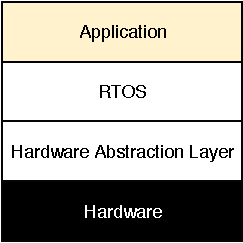
\includegraphics[scale=1]{assets/hal-layers.pdf}
  \caption{\label{fig:hal-layer}Layers around the hardware abstraction layer}
\end{figure}

The figure \ref{fig:hal-layer} shows that the application and the RTOS layers are placed above the HAL, itself just above the device layer.
The application layer talks to the RTOS and the RTOS layer talks to the corresponding HAL depending on the device used.


\paragraph{Pro and cons}
Developers can switch hardware and perform cross-platform testing more easily.
But there is some limitation: The HAL is tied to the hardware and change heavily with it.
Also, there is some limitation using an hardware abstraction layer.
Not all the functionalities from the hardware are available.


\chapter{RTOS Outline}

\section{RIOT OS}
\section{Contiki}
%explain contiki and why we chose it

\subsection{Historic}
\paragraph{}
%https://ieeexplore.ieee.org/stamp/stamp.jsp?tp=&arnumber=1367266
%https://ercim-news.ercim.eu/en76/rd/contiki-bringing-ip-to-sensor-networks
Contiki was created in 2003 by Adam Dunkels. %http://dunkels.com/adam/
At the time, it was the first operating system to provide IP connectivity to sensor networks.
It did so thanks to $\mu$IP, a lightweight TCP/IP stack intended for tiny microcontrollers,
    also developped by Adam Dunkels at the Swedish Institute of Computer Science (now RISE SICS).%https://github.com/adamdunkels/uip

Further developpement of Contiki has been supported by various industries and research institutes 
    such as Texas Instruments, Atmel, Cisco, ENEA, ETH Zurich, Redwire, RWTH Aachen University, 
    Oxford University, SAP, Sensinode, Swedish Institute of Computer Science, ST Microelectronics and Zolertia.
%death?

\subsection{Characteristics and features}
\paragraph{}
The developpement of Contiki started with the need to bring connectivity to small sensor devices with limited capabilities.
By definition, Contiki is not a real-time operating system and has not been designed as such.\\

%memory allocation/stack and kernel/event driven
Contiki operates with the event-driven model.
Processes are implemented as event handlers that run to completion.
An event handler can be defined as a procedure that performs a specific action in response to an event.
Because event handlers cannot block, the same stack can be shared among them.
Also, locking mechanisms are not needed as event handlers do not run concurrently.
Instead of having multiple stacks for multiple threads (which must be over-provisioned or they risk to run out of memory), a single stack can then be used.

This model does not come without problems, as it is sometimes tedious for programmers to manage.
For example, a time-consumming process such as a cryptocraphic operation can monopolize the CPU for quite some time 
    and make the system unable to respond to external events. 
In a preemptive multi-threading system, the computation can be preempted to react to an external event 
    and continue the process later.
To fix this issue, Contiki makes use of an application library that implements preemptible threads.
This library is optional an can be used with programs that explicitly require it.\\

%protothreads
%http://dunkels.com/adam/dunkels05using.pdf
In order to implement its event-driven system, Contiki comes with a mechanism called \textit{protothread}.
The concept of protothreads was also developped by Adam Dunkels with the help of other researchers.
The goal of the protothread programming abstraction is to make it easier for developpers to develop, debug and maintain code written in the event-driven model.

Protothreads can be defined as lightweight stackless threads providing a blocking context on top of an event-driven system.
They can be used to perform non-preemptive concurrency or cooperative multitasking.
Programs written for an event-driven model typically have to be implemented as explicit state machines.
With protothreads, programs can be written in a sequential fashion without designing explicit state machines.

Protothreads do not serve the same purpose as threads for the event-driven model.
The concept has been developped to bring a number of benefits of the multi-threaded programming model into Contiki
    and ease the developpement of applications.\\


%dynamic loading

\subsection{Specificities}
\paragraph{}
%contiki is specific by itself, aims for WSN
%cooja
%rime https://pdfs.semanticscholar.org/9feb/7e0f0d3b507f2f3da60c1b2fea9d5e43449d.pdf